\chapter{Bilag}
\section{Udledning af den ideelle impulsrespons} \label{app1}
For at udlede den ideelle impulsrespons defineres først den ideelle frekvensrespons som følger på baggrund af filterets specifikationer defineret i sektion \ref{ch4_specs}.
\begin{align*}
 H_d(\text{e}^{j\omega})= \begin{cases}
  \text{e}^{-j\omega\frac{M}{2}}, \ \ \ & |\omega| \leq\omega_{c_1} \\
 0, \ \ \ & \omega_{c_1} \leq |\omega| \leq \omega_{c_2} \\
  \text{e}^{-j\omega\frac{M}{2}}, \ \ \ & \omega_{c_2} \leq |\omega| 
\end{cases}
\end{align*}
  
Herudfra bestemmes den ideelle impulsrespons ved hjælp af den inverse Fourier-transformation:
\begin{align*}
h_d[n] &= \frac{1}{2\pi} \left(  \int_{-\pi}^{-\omega_{c_2}} \text{e}^{-j\omega \frac{M}{2}} \cdot \text{e}^{j \omega n} d\omega + \int_{-\omega_{c_1}}^{\omega_{c_1}} \text{e}^{-j\omega \frac{M}{2}} \cdot \text{e}^{j \omega n} d\omega +\int_{\omega_{c_2}}^{\pi} \text{e}^{-j\omega \frac{M}{2}} \cdot \text{e}^{j \omega n} d\omega	\right) \\
&= \frac{1}{2\pi} \left(  \int_{-\pi}^{-\omega_{c_2}} \text{e}^{j\omega \left(n- \frac{M}{2} \right) } d\omega + \int_{-\omega_{c_1}}^{\omega_{c_1}} \text{e}^{j\omega \left(n- \frac{M}{2} \right) }  d\omega + \int_{\omega_{c_2}}^{\pi} \text{e}^{j\omega \left( n-\frac{M}{2} \right) } d\omega	\right).
\end{align*}

Her udnyttes det nu, at der gælder:
\begin{align*}
\int_{-\pi}^{\pi} \text{e}^{j\omega \left(n- \frac{M}{2} \right) }  d\omega =& \int_{-\pi}^{\pi} \cos\left( \omega \left(n-\frac{M}{2}\right)\right)+j \sin \left( \omega \left(n-\frac{M}{2}\right) \right) d\omega \\
=& \left[ \sin\left(\omega \left(n-\frac{M}{2}\right)\right) \right]_{-\pi}^{\pi} \cdot \frac{1}{n- \frac{M}{2}}.
\end{align*}

Således fås:
\begin{align*}
h_d[n]= \frac{1}{\pi \left(n-\frac{M}{2}\right)} \left(\sin\left(\omega_{c_2} \left(n-\frac{M}{2}\right)\right) - \sin\left(\omega_{c_1} \left(n-\frac{M}{2}\right)\right) - \sin\left( \pi\left( n + \frac{M}{2} \right) \right) \right).
\end{align*}

Da sidste led må være $0$ defineres den ideelle impulsrespons som følger:
\begin{align*}
h_d[n]= \frac{1}{\pi \left(n-\frac{M}{2}\right)} \left(\sin\left(\omega_{c_2} \left(n-\frac{M}{2}\right)\right) - \sin\left(\omega_{c_1} \left(n-\frac{M}{2}\right)\right)\right)
\end{align*}

Dette gælder dog kun for $n \neq 0$, og dermed defineres $h_d[0]$ seperat. Hertil anvendes l'Hôspitals regel, som siger, at $\lim \frac{f(x)}{g(x)}=\lim \frac{f'(x)}{g'(x)}$.
\begin{align*}
h_d[0]=& \frac{1}{\pi} \left( \cos\left( \omega_{c_1} \left(n-\frac{M}{2}\right) \right)\omega_{c_1} - \cos\left( \omega_{c_2} \left(n-\frac{M}{2}\right) \right)\omega_{c_2} +  \cos\left(\pi \left( n- \frac{M}{2}\right) \right) \pi \right) \\
=& \frac{1}{\pi}\left( \omega_{c_1} - \omega_{c_2} + \pi \right) \\
=& 1 - \frac{\omega_{c_2}-\omega_{c_1}}{\pi}
\end{align*}

\section{Amplituderespons for Hammingvindue} \label{app2}
\todo{Denne figur mangler som minimum enheder og ``tics'' på akserne. \textregistered}
\begin{figure}[H]
\centering
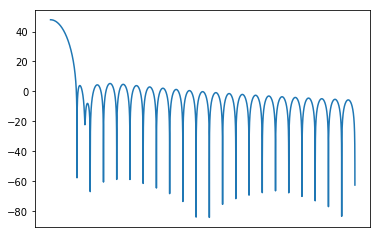
\includegraphics[width=0.7\textwidth]{figures/amplituderespons.png}
\caption{Amplituderespons i dB for Hammingvidue af orden $M=92$.}
\label{fig:amplituderespons}
\end{figure}